\documentclass{scrreprt}

\usepackage{aligned-overset}
\usepackage{amsmath}
\usepackage{amsthm}
\usepackage{amssymb}
\usepackage{bm}
\usepackage[inline,shortlabels]{enumitem}
\usepackage{hyperref}
\usepackage[utf8]{inputenc}
\usepackage{multicol}
\usepackage{mathtools}
\usepackage{pdflscape}
\usepackage{physics}
\usepackage{tabularx}
\usepackage[table]{xcolor}
\usepackage{titling}
\usepackage{fancyhdr}
\usepackage{xfrac}
\usepackage{pgfplots}

\pgfplotsset{compat = newest}
\usepgfplotslibrary{fillbetween}
\usetikzlibrary{calc}


\author{Karsten Lehmann}
\date{SoSe 2025}
\title{Übungsblatt 02\\INF-B-120, Mathematische Methoden für Informatiker}

\setlength{\parindent}{0pt}

\setlength{\headheight}{26pt}
\pagestyle{fancy}
\fancyhf{}
\lhead{\thetitle}
\rhead{\theauthor}
\lfoot{\thedate}
\rfoot{Seite \thepage}

\begin{document}
\paragraph{Ü 2.1} Gegeben ist die Folge $\qty\big(x_n)_{n \in \mathbb{N}}$ mit
  $x_n \coloneqq \frac{n - 4}{2n + 1}$ für $n \in \mathbb{N}$.
\begin{enumerate}[(a)]
\item Bestimmen Sie einen Folgenindex $N_0$ in Abhängigkeit von $\epsilon > 0$
  so, dass $\abs{x_n - \frac{1}{2}} < \epsilon$ für alle $n \geq N_0$ gilt.

  \subparagraph{Lsg.} Sei $\epsilon > 0$ beliebig.
  Dann ist
  \begin{flalign*}
    \abs{x_n - \frac{1}{2}}
    &= \abs{\frac{n - 4}{2n + 1} - \frac{1}{2}} \\
    &= \abs{\frac{2n - 8}{4n + 2} - \frac{2n + 1}{4n + 2}} \\
    &= \abs{\frac{\qty\big(2n - 8) - \qty\big(2n + 1)}{4n + 2}} \\
    &= \abs{-\frac{9}{4n + 2}} = \abs{\frac{9}{4n + 2}} \\
    &< \abs{\frac{9}{4n}} \overset{n > 0} = \frac{9}{4n}
  \end{flalign*}
  Und nun
  \begin{flalign*}
    \epsilon &= \frac{9}{4N_0} && {\Big |} \cdot N_0 && \\
    N_0 \cdot \epsilon &= \frac{9}{4} && {\Big |} \cdot \frac{1}{\epsilon} \\
    N_0 &= \frac{9}{4\epsilon}
  \end{flalign*}

\item Berechnen Sie $N_0$ für $\epsilon = \frac{1}{100}$.

  \subparagraph{Lsg.} $N_0 = \frac{9}{4 \cdot \frac{1}{100}} = \frac{900}{4} = 225$.

\item Ist die Folge konvergent?

  \subparagraph{Lsg.} Es ist nun für jedes $\epsilon > 0$ ein
  $N_0 \in \mathbb{N}$ bekannt, so dass für alle $n > N_0$ gilt
  \[
    \abs{x_n - \frac{1}{2}} < \epsilon
  \]

  $\Rightarrow$ die Folge konvergiert gegen $\frac{1}{2}$.

\end{enumerate}

\newpage
\paragraph{Ü 2.2}
\begin{enumerate}[(a)]
\item Berechnen Sie für die gegebenen Zahlenfolgen
  $\qty\big(x_n)_{n \in \mathbb{N}}$ den Grenzwert $\lim_{n \to \infty} x_n$.
  Verwenden Sie dazu Grenzwertsätze und aus der Vorlesung bekannte Grenzwerte.

  \begin{multicols}{2}
    \begin{enumerate}[(1)]
    \item $x_n \coloneqq \frac{n^3 - 2}{n^4 - n + 4}$
    \item $x_n \coloneqq \frac{4n^2}{\qty\big(n - 2)^3 - n^3}$
    \item $x_n \coloneqq \qty(1 + \frac{3}{4n})^n$
    \item $x_n \coloneqq \qty(\frac{3n - 1}{3n})^{n + 1} + \sqrt[n]{2^{n - 2}}$
    \item $x_n \coloneqq \frac{n^{\frac{2}{n}} + n^2}{2n^2 + 1}$
    \item $x_n \coloneqq \frac{\qty\big(-2)^n}{7^{n + 1}} - \sqrt[n]{3n}$
    \end{enumerate}
  \end{multicols}

  \subparagraph{Lsg.} Es sind
  \begin{enumerate}[(1)]
  \item Es ist
    \begin{flalign*}
      \frac{n^3 - 2}{n^4 - n + 4}
      &= \frac{n^3 \cdot \qty(1 - \frac{2}{n^3})}{n^4 \cdot \qty(1 - \frac{1}{n^3} + \frac{4}{n^2})} \\
      &= \frac{n^3}{n^4} \cdot \frac{1 - \frac{2}{n^3}}{1 - \frac{1}{n^3} + \frac{4}{n^2}} \\
      &= \frac{1}{n} \cdot \frac{1 - \frac{2}{n^3}}{1 - \frac{1}{n^3} + \frac{4}{n^2}}
    \end{flalign*}
    Seien nun $a_n \coloneqq \frac{1}{n}$, $b_n \coloneqq 1 - \frac{2}{n^3}$ und
    $c_n \coloneqq 1 - \frac{1}{n^3} + \frac{4}{n^2}$.

    Dann ist
    \[
      \lim_{n \to \infty} a_n =
      \lim_{n \to \infty} \frac{1}{n} = 0
    \]
    sowie
    \[
      \lim_{n \to \infty} b_n =
      \lim_{n \to \infty} 1 - \frac{2}{n^3} = 1
    \]
    und
    \[
      \lim_{n \to \infty} c_n =
      \lim_{n \to \infty} 1 - \frac{1}{n^3} + \frac{4}{n^2} = 1
    \]

    Da $x_n = a_n \cdot \frac{b_n}{c_n}$, folgt aus den Grenzwertsätzen
    \[
      \lim_{n \to \infty} x_n =
      \qty(\lim_{n \to \infty} a_n) \cdot \frac{\lim_{n \to \infty} b_n}{\lim_{n \to \infty} c_n}
      = 0 \cdot \frac{1}{1} = 0
    \]

  \item Es ist
    \begin{flalign*}
      \frac{4n^2}{\qty\big(n - 2)^3 - n^3}
      &= \frac{4n^2}{n^3 - 6n^2 + 12n - 8 - n^3} \\
      &= -\frac{4n^2}{6n^2 + 12n - 8} \\
      &= -\frac{n^2}{n^2} \cdot \frac{4}{6 + \frac{12}{n} - \frac{8}{n^2}} \\
      &= -\frac{4}{6 + \frac{12}{n} - \frac{8}{n^2}}
    \end{flalign*}

    Seien nun $a_n \coloneqq 4$ und
    $b_n \coloneqq 6 + \frac{12}{n} - \frac{8}{n^2}$.

    Dann ist
    \[
      \lim_{n \to \infty} a_n =
      \lim_{n \to \infty} 4 = 4
    \]
    sowie
    \[
      \lim_{n \to \infty} b_n =
      \lim_{n \to \infty} 6 + \frac{12}{n} - \frac{8}{n^2} = 6
    \]

    Da $x_n = -\frac{a_n}{b_n}$, folgt aus den Grenzwertsätzen
    \[
      \lim_{n \to \infty} x_n =
      -\frac{\lim_{n \to \infty} a_n}{\lim_{n \to \infty} b_n}
      = -\frac{4}{6} = -\frac{2}{3}
    \]

  \item Es ist
    \[
      \qty(1 + \frac{3}{4n})^n
      = \qty(1 + \frac{\sfrac{3}{4}}{n})^n
    \]
    und
    \[
      \lim_{n \to \infty} \qty(1 + \frac{\sfrac{3}{4}}{n})^n = e^{\sfrac{3}{4}}
    \]

  \item Es ist
    \begin{flalign*}
      \qty(\frac{3n - 1}{3n})^{n + 1} + \sqrt[n]{2^{n - 2}}
      &= \qty(\frac{3n}{3n} - \frac{1}{3n})^{n + 1} + \sqrt[n]{2^n \cdot 2^{-2}} \\
      &= \qty(1 - \frac{\sfrac{1}{3}}{n})^{n + 1} + \sqrt[n]{2^n}\sqrt[n]{2^{-2}} \\
      &= \qty(1 - \frac{\sfrac{1}{3}}{n})^n \cdot \qty(1 - \frac{\sfrac{1}{3}}{n}) + 2\sqrt[n]{2^{-2}}
    \end{flalign*}
    Seien nun $a_n \coloneqq \qty(1 - \frac{\sfrac{1}{3}}{n})^n$,
    $b_n \coloneqq \qty(1 - \frac{\sfrac{1}{3}}{n})$,
    $c_n \coloneqq 2\sqrt[n]{2^{-2}}$.

    Dann ist
    \[
      \lim_{n \to \infty} a_n =
      \lim_{n \to \infty} \qty(1 - \frac{\sfrac{1}{3}}{n})^n = e^{-\sfrac{1}{3}}
    \]
    sowie
    \[
      \lim_{n \to \infty} b_n =
      \lim_{n \to \infty} \qty(1 - \frac{\sfrac{1}{3}}{n}) = 1
    \]
    und schließlich
    \[
      \lim_{n \to \infty} c_n =
      \lim_{n \to \infty} 2\sqrt[n]{2^{-2}} = 2
    \]

    Da $x_n = a_n \cdot b_n + c_n$, folgt aus den Grenzwertsätzen
    \[
      \lim_{n \to \infty} x_n = \qty(\lim_{n \to \infty} a_n) \cdot \qty(\lim_{n \to \infty} b_n) +
      \qty(\lim_{n \to \infty} c_n)
      = e^{-\sfrac{1}{3}} \cdot 1 + 2
      = e^{-\sfrac{1}{3}}  + 2
    \]

  \item Es ist
    \begin{flalign*}
      \frac{n^{\frac{2}{n}} + n^2}{2n^2 + 1}
      &= \frac{n^2 \cdot \qty(\frac{n^{\frac{2}{n}}}{n^2} + 1)}{n^2 \cdot \qty(2 + \frac{1}{n^2})} \\
      &= \frac{\frac{1}{n^2} \cdot \sqrt[n]{n}\sqrt[n]{n} + 1}{2 + \frac{1}{n^2}} \\
    \end{flalign*}

    Seien nun $a_n \coloneqq \sqrt[n]{n}$,
    $b_n \coloneqq \frac{1}{n^2}$,
    $c_n \coloneqq \frac{1}{n^2} \cdot \sqrt[n]{n}\sqrt[n]{n} + 1$
    und
    $d_n \coloneqq 2 + \frac{1}{n^2}$.

    Dann ist
    \[
      \lim_{n \to \infty} a_n =
      \lim_{n \to \infty}  \sqrt[n]{n} = 1
    \]
    sowie
    \[
      \lim_{n \to \infty} b_n =
      \lim_{n \to \infty} \frac{1}{n^2} = 0
    \]
    als auch
    \[
      \lim_{n \to \infty} c_n =
      \qty(\lim_{n \to \infty} b_n) \cdot \qty(\lim_{n \to \infty} a_n) \cdot \qty(\lim_{n \to \infty} a_n) + 1 = 1
    \]
    und schließlich
    \[
      \lim_{n \to \infty} d_n =
      \lim_{n \to \infty} 2 + \frac{1}{n^2} = 2
    \]


    Da $x_n = \frac{c_n}{d_n}$, folgt aus den Grenzwertsätzen
    \[
      \lim_{n \to \infty} x_n = \frac{\lim_{n \to \infty} c_n}{\lim_{n \to \infty} d_n}
      = \frac{1}{2}
    \]

  \item Es ist
    \begin{flalign*}
      \frac{\qty\big(-2)^n}{7^{n + 1}} - \sqrt[n]{3n}
      &= \frac{\qty\big(-2)^n}{7^n} \frac{1}{7} - \sqrt[n]{3}\sqrt[n]{n} \\
      &= \qty(-\frac{2}{7})^n \frac{1}{7} - \sqrt[n]{3}\sqrt[n]{n}
    \end{flalign*}
    Seien nun $a_n \coloneqq \qty(-\frac{2}{7})^n$, $b_n \coloneqq \frac{1}{7}$,
    $c_n \coloneqq \sqrt[n]{3}$
    und
    $d_n \coloneqq \sqrt[n]{3}$

    Dann ist
    \[
      \lim_{n \to \infty} a_n =
      \lim_{n \to \infty} \qty(-\frac{2}{7})^n = 0
    \]
    sowie
    \[
      \lim_{n \to \infty} b_n =
      \lim_{n \to \infty} \frac{1}{7} = \frac{1}{7}
    \]
    als auch
    \[
      \lim_{n \to \infty} c_n =
      \lim_{n \to \infty} \sqrt[n]{3} = 1
    \]
    und schließlich
    \[
      \lim_{n \to \infty} d_n =
      \lim_{n \to \infty} \sqrt[n]{n} = 1
    \]


    Da $x_n = a_n \cdot bn + c_n \cdot d_n$, folgt aus den Grenzwertsätzen
    \[
      \lim_{n \to \infty} x_n = \qty(\lim_{n \to \infty} a_n)\qty(\lim_{n \to \infty} b_n) +
      \qty(\lim_{n \to \infty} c_n)\qty(\lim_{n \to \infty} d_n) = 1
    \]
  \end{enumerate}

\item Untersuchen Sie für zwei beliebige Polynomfunktionen
  $p\qty\big(x) = a_mx^m + \ldots + a_1x + a_0$ und
  $q\qty\big(x) = b_kx^k + \ldots + b_1x + b_0$ mit $q\qty\big(n) \ne 0$ für
  $n \in \mathbb{N}$ die Konvergenz der Zahlenfolge $\qty\big(x_n)$ mit
  $x_n \coloneqq \frac{p\qty\big(n)}{q\qty\big(n)}$ in Abhängigkeit vom
  Verhältnis der Grade von $p\qty\big(x)$ und $q\qty\big(x)$.

  \subparagraph{Lsg.} Die beiden Polynomfunktionen können alternativ als
  \[
    p\qty\big(x) = x^m \cdot \qty(a_m + a_{m - 1} \frac{1}{x} +
    \ldots + \frac{a_1}{x^{m - 1}} + \frac{a_0}{x^m})
  \]
  und
  \[
    q\qty\big(x) = x^k \cdot \qty(b_k + b_{k - 1} \frac{1}{x} +
    \ldots + \frac{b_1}{x^{k - 1}} + \frac{b_0}{x^k})
  \]
  schreiben.

  Dann ist
  \begin{flalign*}
    x_n &= \frac{n^m \cdot \qty(a_m + a_{m - 1} \frac{1}{n} + \ldots + \frac{a_1}{n^{m - 1}} + \frac{a_0}{n^m})}{n^k \cdot \qty(b_k + b_{k - 1} \frac{1}{n} + \ldots + \frac{b_1}{n^{k - 1}} + \frac{b_0}{n^k})} \\
    &= \frac{n^m}{n^k} \cdot \frac{a_m + a_{m - 1} \frac{1}{n} + \ldots + \frac{a_1}{n^{m - 1}} + \frac{a_0}{n^m}}{b_k + b_{k - 1} \frac{1}{n} + \ldots + \frac{b_1}{n^{k - 1}} + \frac{b_0}{n^k}}
  \end{flalign*}

  Dabei ist bereits ersichtlich, dass
  \[
    \lim_{n \to \infty} \frac{a_m + a_{m - 1} \frac{1}{n} + \ldots + \frac{a_1}{n^{m - 1}} + \frac{a_0}{n^m}}{b_k + b_{k - 1} \frac{1}{n} + \ldots + \frac{b_1}{n^{k - 1}} + \frac{b_0}{n^k}}
    = \frac{a_m}{b_k}
  \]

  \newpage
  Für $\frac{n^m}{n^k}$ müssen hingegen 3 Fälle unterschieden werden:
  \begin{itemize}
  \item[$k = m$:] Es ist $\frac{n^m}{n^k} = 1$ und
    \[
      \lim_{n \to \infty} x_n = \frac{a_m}{b_k}
    \]

  \item[$k > m$:] Offensichtlich ist $\frac{n^m}{n^k} = \frac{1}{n^{k - m}}$ mit
    $k - m > 0$ und
    \[
      \lim_{n \to \infty} x_n = 0 \cdot \frac{a_m}{b_k} = 0
    \]

  \item[$k < m$:] Nach Voraussetzung ist $\frac{a_m}{b_k} \ne 0$ und somit
    hat $\frac{n^m}{n^k} \cdot \frac{a_m}{b_k}$ keine obere Schranke und die
    Folge divergiert.
  \end{itemize}
\end{enumerate}

\paragraph{Ü 2.3}
\begin{enumerate}[(a)]
\item Betrachtet wird die Zahlenfolge $\qty\big(x_n)$ mit
  $x_n \coloneqq \frac{\qty\big(10 - n)\cos\qty\big(1 + n^2)}{1 + n^2}$,
  $n > 0$.
  Für die reelle Funktion
  $f\qty\big(x) \coloneqq \frac{\qty\big(10 - x)\cos\qty\big(1 + x^2)}{1 + x^2}$
  gilt offenbar $f\qty\big(n) = x_n$ für alle $n \in \mathbb{N}$.
  Veranschaulichen Sie den Graph von $f$.
  Bestimmen Sie mit Hilfe des Quetschlemmas den Grenzwert
  $\lim_{n \to \infty} x_n$.

  \subparagraph{Lsg.} Der Graph:

  \begin{tikzpicture}[scale=1]
    \begin{axis}[
      axis equal image,
      axis x line=center,
      axis y line=center,
      grid=both,
      samples=200,
      xmin=-5.5,
      xmax=5.5,
      xtick distance=1,
      ymin=-5.5,
      ymax=5.5,
      ytick distance=1,
    ]
      \addplot[domain=-5:5, smooth] { ((10 - \x) * cos(deg(1 + \x * \x))) / (1 + \x * \x) };
    \end{axis}
  \end{tikzpicture}

  Seien $a_n \coloneqq -\frac{10 - n}{1 + n^2}$ und
  $b_n \coloneqq \frac{10 - n}{1 + n^2}$.
  Nun ist die Cosinus-Funktion von 1 und -1 begrenzt, daher gilt
  \[
    a_n \leq x_n \leq b_n
  \]
  Nun ist
  \begin{flalign*}
    \lim_{n \to \infty} \pm \frac{10 - n}{1 + n^2}
    &= \lim_{n \to \infty} \pm \frac{n^2 \cdot \qty\big(\frac{10}{n^2} - \frac{1}{n})}{n^2 \cdot \qty\big(\frac{1}{n^2} + 1)} \\
    &= \lim_{n \to \infty} \pm \frac{\frac{10}{n^2} - \frac{1}{n}}{\frac{1}{n^2} + 1} \\
    &= \pm \frac{\qty(\lim_{n \to \infty} \frac{10}{n^2} - \frac{1}{n})}{\qty( \lim_{n \to \infty}\frac{1}{n^2} + 1)} \\
    &= \frac{0 - 0}{0 + 1} = 0
  \end{flalign*}
  Und aus dem Quetschlemma folgt $\lim_{n \to \infty} x_n = 0$
\item Verwenden Sie das Quetschlemma, um für die reellen Zahlenfolgen
  $\qty\big(x_n)$ mit
  \begin{multicols}{2}
    \begin{enumerate}[(1)]
    \item $x_n = \sqrt[n]{2 + n^{-1}}, n > 0$
    \item $x_n = \sqrt[n]{n + 3}$
    \end{enumerate}
  \end{multicols}
  den Grenzwert zu berechnen.

  \subparagraph{Lsg.}
  \begin{enumerate}[(1)]
  \item Betrachte $n^{-1}$ und stelle fest, dass $0 < n^{-1} \leq 1$ für alle
    $n \in \mathbb{N}$.

    Seien nun $a_n \coloneqq \sqrt[n]{2}$ und $b_n \coloneqq \sqrt[n]{3}$.
    Dann ist $a_n < x_n \leq b_n$.

    Da $\lim_{n \to \infty} \sqrt[n]{a} = 1$ für alle $a \in \mathbb{R}, a > 0$
    folgt aus dem Quetschlemma $\lim_{n \to \infty} x_n = 1$.

  \item Seien $a_n \coloneqq \sqrt[n]{n}$ und
    $b_n \coloneqq \sqrt[n]{3n} = \sqrt[n]{3}\sqrt[n]{n}$.
    Dann ist (für $n > 1$) $a_n \leq x_n \leq b_n$ und da
    \[
      \lim_{n \to \infty} \sqrt[n]{n} = 1
      \text{ sowie }
      \lim_{n \to \infty} \sqrt[n]{3}\sqrt[n]{n} =
      \qty(\lim_{n \to \infty} \sqrt[n]{3})\qty(\lim_{n \to \infty} \sqrt[n]{n}) =
      1 \cdot 1 = 1
    \]
    folgt aus dem Quetschlemma $\lim_{n \to \infty} x_n = 1$.
  \end{enumerate}

\end{enumerate}
\end{document}
